\documentclass{article}

\usepackage[margin=1.15in]{geometry}
\usepackage{natbib}

% Tikz for flow chart
%https://www.overleaf.com/learn/latex/LaTeX_Graphics_using_TikZ%3A_A_Tutorial_for_Beginners_(Part_3)%E2%80%94Creating_Flowcharts
\usepackage{tikz}
\usetikzlibrary{shapes.geometric, arrows}
\tikzstyle{startstop} = [rectangle, rounded corners, minimum width=1.75cm, minimum height=1cm,text centered, draw=black]
\tikzstyle{io} = [trapezium, trapezium left angle=70, trapezium right angle=110, minimum width=1.75cm, minimum height=1cm, text centered, draw=black, fill=blue!30]
\tikzstyle{process} = [rectangle, minimum width=1.75cm, minimum height=1cm, text centered, draw=black]
\tikzstyle{decision} = [diamond, minimum width=1.75cm, minimum height=1cm, text centered, draw=black]
\tikzstyle{arrow} = [thick,->,>=stealth]



\title{GromStole: A Pipeline for SARS-CoV-2 Variant Detection in Wastewater Samples}
\author{Art Poon, Devan Becker, Gopi Gugan, Erin Brintnell, Art Poon (again)}
\date{\today}


% Tighter lists
\newenvironment{tightemize}
{ \begin{itemize}
    \setlength{\itemsep}{0pt}
    \setlength{\parskip}{0pt}
    \setlength{\parsep}{0pt}     }
{ \end{itemize}                  } 

% TODO: Track down my references


\begin{document}
\maketitle

Right now this is a skeleton. 
The plan is to expand each bullet into \emph{exactly} one paragraph. 
We'll see how well this plan works out.


\section*{Abstract}

\section{Introduction}

% Background info and importance
It is clinically and logistically important to know which ``variants'' of SARS-CoV-2 are spreading in a given region so that the correct action can be taken for the individual and for the government.
Genetic sequencing of SARS-CoV-2 genomes from patients is costly and requires coordination between clinics, sequencing labs, and some central organizing agency \citep{needed}, which means that a small percentage of COVID-19 patients have samples of the virus taken for sequencing.
Sequences acquired this way are strongly affected by sampling bias - in general, patients at higher risk of having a variant of interest are preferentially sampled \citep{needed}.
For this reason, detection of variants in wastewater provides an attractive alternative that allows for unbiased sampling and continuous monitoring. 


\begin{tightemize}
    \item Other papers that have done wastewater monitoring for detection/amount of any virus
    \item Other papers that have done wastewater monitoring for detection/amount of SARS-CoV-2
    \item Other papers that have done wastewater monitoring for \emph{variants}
\end{tightemize}

% Terminology - variant versus lineage
Before we continue, we make a brief note on terminology. 
``Variant of Concern'' (VoC) and ``Variant of Interest'' (VoI) are terms used by the World Health Organization \citep[WHO, ][]{needed} to refer to collections of SARS-CoV-2 genomes (as defined using a phylogenetic tree) that are clinically or epidemiologically interesting. 
The term ``lineage'' is used by the Pangolin team to refer categorization of genomes chosen based on a phylogeny \citep{needed}.
In general, a VoC or VoI corresponds to exactly one lineage in the Pangolin classification system.
In this paper, we use ``variant'' to refer to a particular lineage that we are searching for in a wastewater sample; otherwise ``variant'' and ``lineage'' are used interchangeably.
We use ``variant of interest'', in all lower case, to refer to the variant that we are interested in detecting, rather than the WHO's definition.

% Statement of our goals, including output format and basic modelling
% Representative mutations
We have developed a pipeline that uses open access data to determine the relative abundance of mutations across all lineages and then use this information to detect variants of interest in samples of wastewater.
Here, we provide a broad overview of the pipeline before delving into the specifics.

The first step is to determine which mutations we are looking for in the wastewater samples.
The pipeline begins by aligning all data (open access as well as the wastewater samples) to a reference sequence and recording a set of mutations for each observed sequence or short read.
The sets of mutations for each known lineage are combined so that we can easily look up mutations unique to a lineage.
The relative abundance of mutations across all lineages is important to reduce the chance of false positives, \emph{i.e.} when a variant of interest shares mutations with another lineage.
Before attempting detection, we filter out the mutations of a variant that are common in the population and/or rarely observed in the variant.
This pipeline leaves us with a list of representative mutations for our variant and the number of times that each mutation could have been observed (it is also possible to circumvent this step and provide a custom list of mutations to be detected).

% Coverage
In addition to the number of times a mutation was observed, we also record the number of times each position on the reference genome was observed; that is, the number of short reads that had coverage at each position.
The coverage is found at the position of every mutation in the variant of interest; if a particular mutation was not observed in a sample, it is still important to know the coverage at that position.
If the position of a mutation has low (or zero) coverage, then the lack of observations of this mutation is not strong evidence of either presence or absence.

% Modelling
Given the list of mutations, we use a simple binomial model to detect the variant.
There is still a risk that some of the representative mutations for the variant have arisen independently in other lineages.
Furthermore, there is the chance that mutations have arisen due to sequencing error \citep{needed}.
Because of this, we use a binomial model that assumes a constant proportion for each mutation but allows for variance around this proportion.
The proportion should be carefully interpreted as the average proportion of each representative mutation, not as the proportion of genome sequences in the wastewater that are consistent with the variant of interest.
The confidence interval of the proportion parameter is compared to an assumed sequencing error for the Next Generation Sequencing (NGS) machines, and any confidence interval that is entirely above the assumed error is declared a potential detection of the variant.


% TODO: Grey boxes denoting section?
\begin{figure}[h!]
\centering
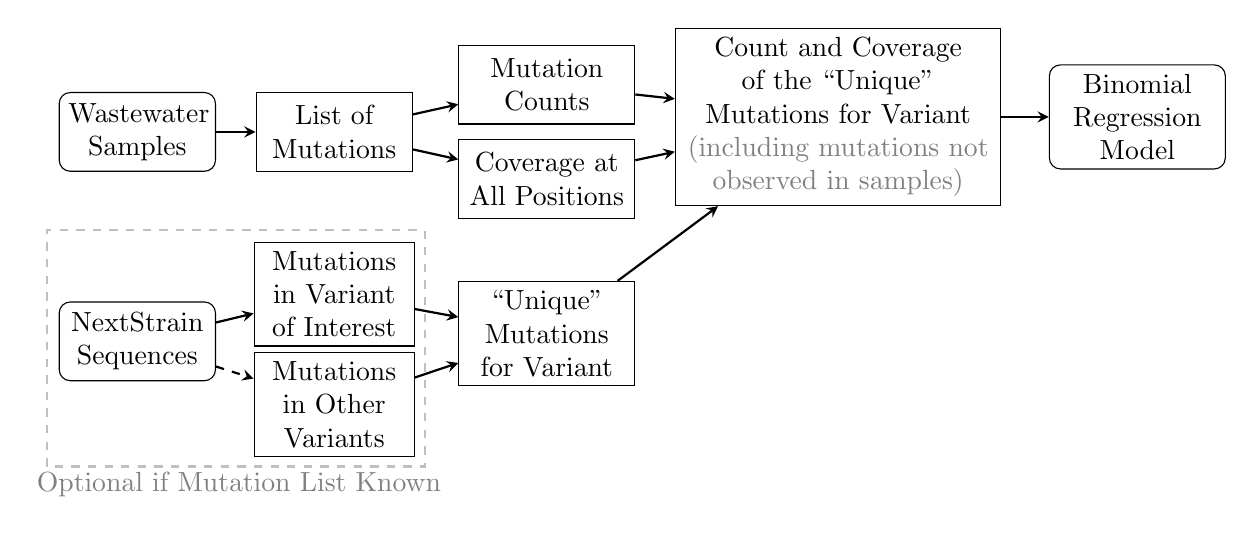
\begin{tikzpicture}[node distance=1cm]
% Process Samples
\node (waste) [startstop, text width=1.75cm] {Wastewater Samples};
\node (wlist) [process, text width=1.75cm, right of=waste, xshift=1.5cm] {List of Mutations};
\draw [arrow] (waste) -- (wlist);
\node (wmut) [process, right of=wlist, xshift=1.7cm, yshift=0.6cm, text width=2cm] {Mutation Counts};
\draw [arrow] (wlist) -- (wmut);
\node (wcov) [process, below of=wmut, yshift=-0.2cm, text width=2cm] {Coverage at All Positions};
\draw [arrow] (wlist) -- (wcov);

% Gather Unique mutations (in a grey rectangle)
\node (nextstrain) [startstop, text width=1.75cm, below of=waste, yshift=-1.66cm] {NextStrain Sequences};
\node (nsmut) [process, right of=nextstrain, xshift=1.5cm, text width=1.8cm, yshift=0.6cm] {Mutations in Variant of Interest};
\node (nsomi) [process, below of=nsmut, text width=1.8cm, yshift=-0.4cm] {Mutations in Other Variants};
\draw [arrow] (nextstrain) -- (nsmut);
\draw [thick, dashed,->,>=stealth] (nextstrain) -- (nsomi);
\draw [color=lightgray, thick, dashed](-1.15, -4.25) rectangle (3.65,-1.25);
\node at (-1.2, -4.25) [below=2.3mm, right=-2mm] {\textcolor{gray}{Optional if Mutation List Known}};
% Outside rectangle
\node (uniques) [process, right of=nsmut, yshift=-0.5cm, xshift=1.7cm, text width=2cm] {``Unique'' Mutations for Variant};
\draw [arrow] (nsmut) -- (uniques);
\draw [arrow] (nsomi) -- (uniques);

% Used \hyphencahr\font=-1 to prevent words from hyphenating and wrapping to next line
% Used \quad to control which words wrap to next line
\node (detect) [process, right of=uniques, yshift=2.75cm, xshift=2.7cm, text width=3.9cm] {\hyphenchar\font=-1 Count and Coverage of the ``Unique'' Mutations for Variant \quad\quad\quad\textcolor{gray}{(including mutations not observed in samples)}};
\draw [arrow] (uniques) -- (detect);
\draw [arrow] (wmut) -- (detect);
\draw [arrow] (wcov) -- (detect);

% End
\node (model) [startstop, right of=detect, xshift=2.8cm, text width=2cm] {Binomial Regression Model};
\draw [arrow] (detect) -- (model);
\end{tikzpicture}
\caption{The structure of our pipeline.
Wastewater samples are processed to find the number of times each mutation is observed along with the coverage at every position (relative to the reference genome).
This information is combined with a list of mutations believed to be unique to the variant of interest (possibly from counts of mutations in known lineages from NextStrain).
It is important to have the coverage for the position of each ``unique'' mutation, regardless of whether this was observed in the wastewater samples.
The proportion is found via a binomial regression model.}
\end{figure}


\section{Data Processing}

\subsection{Input Format}

% Context of data
Our pipeline assumes that data come from wastewater samples processed according to the ARTIC pipeline \citep{needed} on the Illumina NGS platform \citep{needed}, although the pipeline can be modified for other platforms.
The expected format is a FASTQ file \citep{needed}, where each entry represents one short read from the amplicons specified in ARTIC V3. %TODO: Does it have to be V3? We didn't end up using the amplicons anywhere.
These files are expected to follow the FASTQ specification, with a sequence information row, the sequence itself, a plus sign, then the Phred score \citep{needed}.
A reference genome is also required for data processing.
We use Wuhan-1 \citep{needed} as the default, but the pipeline allows for specification by the user.


\begin{figure}[h!]
\begin{verbatim}
First Read          Second Read
@Read 1             @Read 1
GGAGTA              CGGAGT
+                   +
!>ACBA              >>CBA!
@Read 2             @Read 2
TCGAT               TTGAT
@Read 3             @Read3  
TCGCTC              TCGCTC
@Read 4             @Read4
TCGCT               AACACCAT
@Read 5             @Read 5
CTCAGTACA           CTCAGTCCA
\end{verbatim}
\caption{Example paired-end FASTQ files, where each column is a separate file.
Phred scores for reads 2-5 are not shown to save space.}
\label{short-reads}
\end{figure}



\begin{tightemize} 
    \item TODO: Required modifications for other platforms?
\end{tightemize}

\subsection{Parsing FASTQ files}

% Description of desired output format
The purpose of this step of the pipeline is to convert the input FASTQ files into a list of mutations for each read and the coverage at each position of the reference genome.
The mutation list allows us to search for the mutations that we are interested in.
For a mutation that was not observed in the data, the coverage at each position allows us to determine whether it wasn't observed because there was low or zero coverage at the position where it would be or if there was sufficient coverage to detect it but it wasn't present.
The \texttt{minimap2.py} script accepts a FASTQ file (or pair of FASTQ files for paired-end reads) as well as a reference genome and outputs \texttt{mutations.csv} and \texttt{coverage.csv}.

% Parsing into features by mapping to reference
The \texttt{mutations.csv} file contains the mutation description (described below), the frequency of that mutation, the position relative to the reference, and the coverage at that position.
This structure is demonstrated in Figure \ref{mapped}.
As a demonstration, an intermediary step in finding he mutations and coverage of the short reads in Figure \ref{short-reads} is shown in Table \ref{aligned}.


The mutation description includes the alteration relative to the reference, which is labelled as \texttt{$\sim$}, \texttt{+}, or \texttt{-} for polymorphism, insertion, or deletion, respectively.
For polymorphisms, the nucleotide from the reference genome is not included in the label but the new nucleotide is.
For insertions, the added nucleotides are listed.
For deletions, the number of deletions is recorded.
The ``fields'' in the description are separated by the pipe character, \texttt{|}.
This is to avoid ambiguity in deletions, e.g. whether \texttt{-9911} is one deletion at position 991 or 11 deletions at position 99.

\begin{table}[h!]
\begin{tabular}{llll}
Read & Sequence & Mutations & Coverage \\\hline
Reference & \texttt{TCGCTCGGATTACAT} &  &  \\
Position & \texttt{012345678901234} && \\\hline
1         & \texttt{-----CGGA\textcolor{red}{G}TA---} & \texttt{$\sim$|9|G} & \texttt{[[5,11]]}\\
2         & \texttt{----TCG\textcolor{red}{-}AT-----} & \texttt{-|8|1} & \texttt{[[4,9]]}\\
3         & \texttt{TCGCTC---------} & & \texttt{[[0,5]]}\\
4         & \texttt{TCGCT------A\textcolor{red}{ACAC}CAT} & \texttt{+|11|ACAC} & \texttt{[[0,5], [11,14]]}\\
5         & \texttt{---CTC\textcolor{red}{--}A\textcolor{red}{G}TACA-} & \texttt{-|6|2}, \texttt{$\sim$|9|G}& \texttt{[[3,13]]}\\\hline
Coverage & \texttt{222344333323221} &&
\end{tabular}
\caption{Merging the short reads in Figure \ref{short-reads} and aligning to the reference to the determine the mutation list and coverage.
Our methods for merging the paired-end reads are detailed in the text.
The alignments are pairwise, so the insertions in Read 4 do not affect the alignment of the other reads.
The final row is the observed number of reads at each position on the reference (again, the insertions of Read 4 do not affect the position in the reference; the final \texttt{CAT} are in positions 12, 13, and 14).}
\label{aligned}
\end{table}

%TODO: Get verbatim next to each other, with captions: https://stackoverflow.com/questions/2983839/latex-two-captioned-verbatim-environments-side-by-side
%TODO: anonymize 
\begin{figure}[h!]
\begin{verbatim}
position,label,mutation,frequency,coverage
9,~|9|G,None,0.4,3
6,-|6|2,0.2,3
8,-|8|1,0.2,3
11,+|11|ACAG,0.2,3
\end{verbatim}
\caption{\texttt{mapped.csv}, the mutation list calculated from Table \ref{aligned}.
The frequency column is calculated as the number of reads where the given observation was observed divided by the number of short reads.}
\label{mapped}
\end{figure}

\begin{figure}[h!]
\begin{verbatim}
position,coverage
0,2
1,2
2,2
3,3
4,4
...,...
\end{verbatim}
\caption{\texttt{coverage.csv}. 
This file can be used to look up the coverage at positions where a mutation of interest was not found in the data.}
\label{coverage}
\end{figure}

% Dealing with paired-end data: coverage
There were several decisions that needed to be made to determine the observed coverage and mutations.
For instance, in Read 1, the first read covers positions 6 to 11 but the second covers positions 5 to 10, relative to the reference genome.
We merge these two reads and chose to take the union of the coverage.
This means that position 5 only had one observation from Read 1 while position 6 had two observations, but they're both being treated as a full observation.
This merging strategy is necessary for an accurate evaluation of the frequency of each mutation; if the mutation is only observed on one short read and the other read has no coverage at that position, the mutation is still treated as one mutation so the coverage must count as one observation towards the total.

In Table \ref{aligned}, note that the \texttt{-} characters in read 4 are black, not red, despite being between called bases.
In our example here, these are unobserved positions rather than deletions --- Figure \ref{short-reads} shows that there is no overlap between Read 4 in the two FASTQ files.
This is not uncommon; the sequencing platform starts reading from either end of the amplicon, but does not read far enough in either direction to overlap.

% Dealing with paired-end data: mutations in one or both
Read 5 in Figure \ref{short-reads} demonstrates another challenge for paired-end reads: they may disagree on the base calls.
In particular, the 9th base in the short read is A in the first read and C in the second.
We chose to only count mutations if they appear in both short reads, hence why this mutation is not recorded in Table \ref{aligned}.
This has the side effect of putting a higher burden of proof on mutations in positions with coverage from both short reads.
Again, this is necessary to ensure that there is one full observation of coverage at the position of each full observation of a mutation, without resorting to fractional observations.

The python script \texttt{minimap2.py} takes a pair of FASTQ files as input (along with a reference genome) and produces both \texttt{mapped.csv} (Figure \ref{mapped}) and \texttt{coverage.csv} (Figure \ref{coverage}).
% TODO: Add to this paragraph


\subsection{Frequency of ``Unique'' Mutations}

% Motivation
Our binomial regression model estimates a proportion based on all of the supplied mutations.
Any mutation that is present in other lineages will artificially inflate our estimated proportions.
Prior to modelling, we must ensure that our set of mutations is common in the variant of interest but uncommon in other lineages.
We put ``unique'' in quotation marks because we accept that each mutation might be present in other lineages in small numbers, might arise due to chance, or might arise due to sequencing error.
In this section we detail our current process for creating a list of mutations to be used in the modelling stage, starting by acquiring a collection of sequences and processing them to find the frequency of each mutation within each lineage.

\subsubsection{Frequency of Mutations}

% Motivation/processing
Our first step is to obtain a large collection of sequences.
We obtain this as a large FASTA file, available publicly from NextStrain.
We immediately process each sequence into a list of mutations using the same methods as \texttt{minimap2.py}.
As we stream through the sequences, we record the lineage assigned to the sequence.
For each lineage, we start with an empty list and either add a mutation to the list when it is observed in that lineage or increment the count of that mutation if it was already observed.
Note that the record for a given lineage only contains mutations that have counts larger than 0; we do not need to add all mutations to all lineage records.
Each record also contains the \emph{frequency} of each mutation within a lineage, i.e., the percent of sequences labelled with a lineage that contained a given mutation.
When we refer to frequency of a mutation, we mean within a lineage rather than across all lineages.
This is stored in a compressed \texttt{json} file format, with entries for each lineage, each of that lineage's mutations, and the frequency of each mutation.
The downloading and processing of NextStrain data is handled by \texttt{retrieve-nsgb.py}.



\subsubsection{Variant-Specific Mutations}

With a list of mutations and their frequencies within lineages we are able to determine which mutations are ``unique'' to the variant of interest.
We have written a python script to determine all of the mutations for a given set of variants and report the frequency of those mutations in all available lineages (including the variants of interest).
We refer to ``unique'' mutations as those which are present in more than 95\% of the variant(s) of interest and also present in fewer than 5\% of the any other lineage available on NextStrain.
Recall that these frequencies refer to the number of mutations among sequences labelled with a specific lineage, rather than across lineages.
The word ``unique'' has appeared in quotation marks because we allow for the possibility of another lineage with 5\% of the sequences in that lineage having that mutation, so it is not strictly unique. 

The scripts that we have written allow for a set of variants to be studied concurrently.
This is particularly useful when investigating a variant such as Omicron, which has pangolin label B.1.1.529 and also has sublineages BA.1 and BA.2 at time of writing.
Since our analyses currently only considering one variant at a time, these are saved to separate files for processing later in the pipeline.


\begin{figure}[ht!]
\vspace{2cm}
\centering
\emph{Scatterplot of background frequency versus omicron frequency, coloured according to Omicronians(95,5), possibly with different shapes to denote the sub-lineages.}
\vspace{2cm}
\caption{Frequency of mutations in all variants versus in one specific variant. By comparing these two frequencies, we are able to specify variants that should only be common in our variant of interest.}
\label{fig:mutation_frequency}
\end{figure}






\section{Single Variant Detection}

Our method of variant detection is uses every mutation that we have identified.
We use a binomial model which assumes that each mutation should have approximately the same prevalence in the data and any deviation is simply random chance.
In particular, the assumption is that there are a fixed number of SARS-CoV-2 genomes in the wastewater from which the sample was drawn, with a fixed proportion ($p$) of the variant of interest, and parts of the sequences are lost completely at random.
The advantage of the parametric assumption is that we can calculate a confidence interval for the range of possible proportions in the population.

The model is set up as follows.
For mutation $i=1$ to $n$, the count for mutation $i$, and the coverage for mutation $i$,
\begin{equation}
\textrm{count}_i \sim \textrm{Binom}(p, \textrm{coverage}_i)
\end{equation}
In the above model, note that the proportion $p$ is the same for all mutations.
This model is implemented in the R programming language using the \texttt{glm()} function.

Even with our best attempt at defining our mutations will inevitably result in a mismatch between our chosen mutations and the mutations present in the variant of interest.
This is due to the random variation in mutations from the natural evolution of SARS-CoV-2, which means that lineages that are not our variant of interest may gain mutations in our ``unique'' mutations.
Because of this, we allow for extra variation in the proportion by fitting a quasi-binomial model \cite{needed}. % TODO: Reference from https://www.slu.se/globalassets/ew/org/centrb/statisticsslu/workshops/2014/overdispersion.pdf 
This model produces the same estimate of the proportion but allows for larger estimates of the variance than would be possible in the binomial model and hence returns a larger confidence interval. 

We use the confidence intervals to make our conclusion.
Under the conservative assumption that Illumina sequencing methods have a sequencing error of 1\%, so we only claim detection if the lower bound of our confidence interval is larger than 0.01.






\section{Example Usage}

\begin{tightemize}
    \item Description of our particular data collection methods and project goals
    \item With permission, description of the results for Omicron in samples with good metadata.
\end{tightemize}

\begin{figure}[ht!]
\vspace{2cm}
\centering
\emph{Bar plots with confidence bands for GLM results, ordered by time.}
\vspace{2cm}
\caption{Results of the binomial GLM on our available data. The proportion of observed Omicron mutations appears to have increased slightly over time, but still does not reach the 1\% proportion required for us to confidently assert the presence of Omicron.}
\label{fig:binomial_results}
\end{figure}


\section{Discussion and limitations}

\begin{tightemize}
    \item The method is statistically good.
    \item The method is practically good.
    \item Can be modified to different wastewater data formats.
    \item We cannot detect unknown variants with this method.
\end{tightemize}


\bibliography{methods_bib}{}
\bibliographystyle{abbrvnat}

\end{document}

